% \section{System-Level Analysis} \label{sec:results}
\section{Baseline I/O Performance} \label{sec:results}

Because variation in peak I/O performance is known to be caused by different I/O access patterns~\cite{Lofstead2010,Uselton2010,Xie2012}, we first establish the baseline performance variation of each benchmark on each system tested.
we define the \emph{fraction of peak performance} as the mean I/O bandwidth (performance) of a job divided by the maximum performance observed for all jobs \emph{of the same I/O motif} as listed in Table \ref{tab:bench-config} and whether the job did reads or writes.
For example, the fraction peak performance for a HACC write test is only normalized to the maximum performance of all other HACC write tests on the same file system.

The distribution of fraction peak performance, shown in Figure~\ref{fig:perf-summary-boxplots-motif}, reveals that the degree of performance variation \emph{within} each application varies with each file system.
For example, the HACC write workload is susceptible to a long tail of performance degradation on mira-fs1 despite that file system's overall lower variation as evidenced by the distance between all I/O motifs' whiskers relative to the Edison file systems.
Edison's scratch3 also demonstrates very broad performance variation for the VPIC write workload, contrasting with the relatively narrow performance variation of this application on other systems.

\begin{figure}[t]
    \centering
    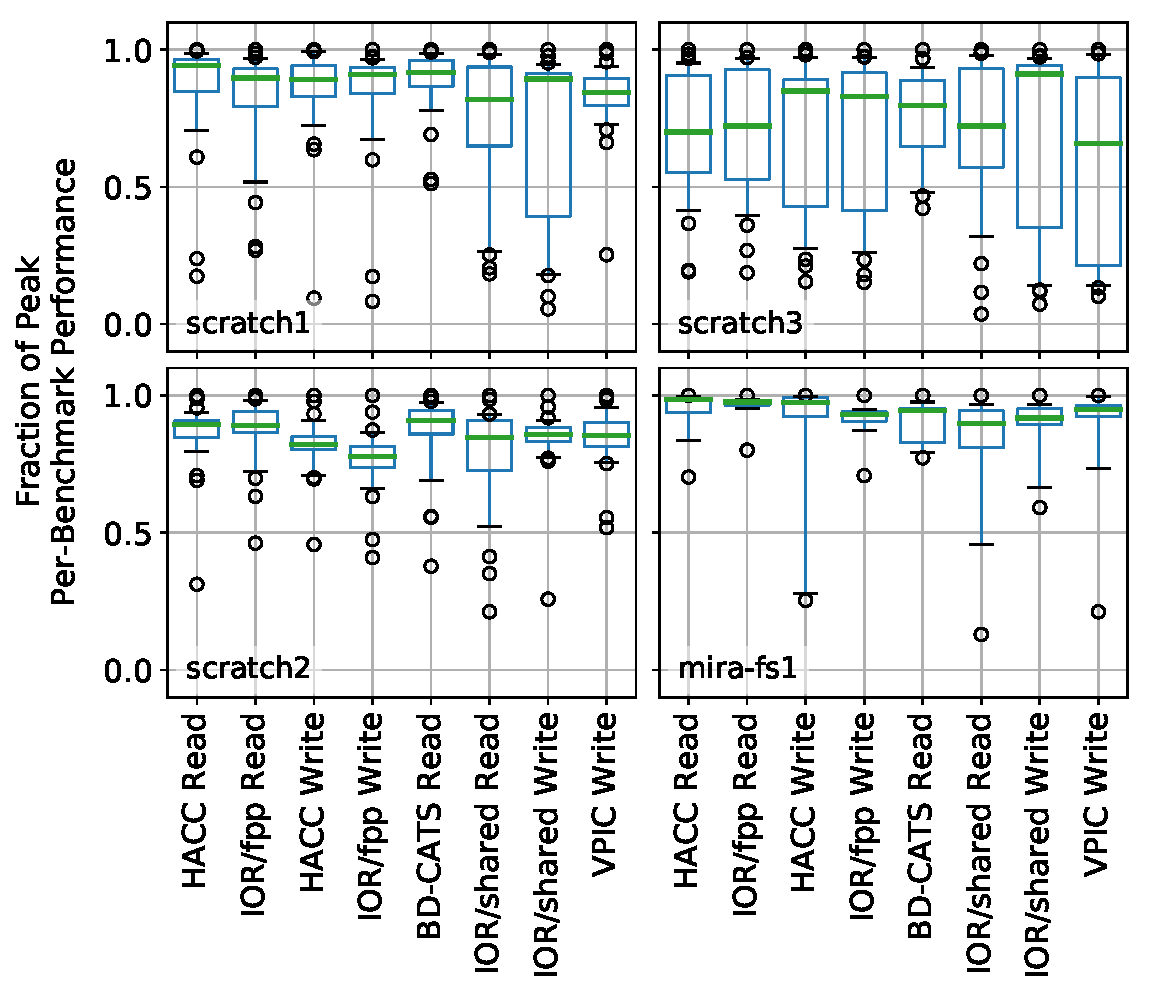
\includegraphics[width=1.0\columnwidth]{figs/perf-boxplots.pdf}
    \caption{I/O performance for all file systems tested grouped by test
    applications and read/write mode.  Whiskers represent the 5th and 95th
    percentiles.}
    \label{fig:perf-summary-boxplots-motif}
\vspace{-.2in}
\end{figure}

We can conclude from this that performance variability is the result of factors intrinsic to the application \emph{and} factors intrinsic to the file system;
different I/O motifs result in different levels of performance \emph{and} variability.
Furthermore, these behaviors are not a function of the parallel file system architecture either; all Edison file systems are Lustre-based, yet Figure~\ref{fig:perf-summary-boxplots-motif} shows a marked difference in variability between scratch1/scratch2 and scratch3.
Thus, these differences in performance variation must be a function of their different hardware configurations, their specific I/O patterns, or a combination of both.
This finding underscores the importance of examining multiple sources of I/O characterization data (e.g., application-level and server-side) in concert to develop a full understanding of I/O performance.

%%%%%%%%%%%%%%%%%%%%%%%%%%%%%%%%%%%%%%%%%%%%%%%%%%%%%%%%%%%%%%%%%%%%%%%%%%%%%%%%
\section{Integrated Analysis} \label{sec:results/umami}
%%%%%%%%%%%%%%%%%%%%%%%%%%%%%%%%%%%%%%%%%%%%%%%%%%%%%%%%%%%%%%%%%%%%%%%%%%%%%%%%

With an understanding of the baseline performance variation on each system and application tested, we can then combine the application performance data derived from the sources described in Section \ref{sec:methods} to better understand how the factors extrinsic to the application contribute to performance variation.

I/O bandwidth contention from other jobs is an intuitive source in I/O performance variation, so we define the \emph{bandwidth coverage factor} ($\mathit{CF}_{\mathit{bw}}$) of a job $j$ to quantify the effects of such competing I/O traffic:

\begin{equation} \label{eq:cf}
    \mathit{CF}_{\mathit{bw}}(j) = \frac{N_{\textup{bytes}}^{\textup{Darshan}}(j)}
    {\sum_{t,s}^{\textup{time,servers}}
    \left [ N_{\textup{bytes}}^{\textup{LMT,ggiostat}}(t,s) \right ] }
\end{equation}
%
where 
$N_{\textup{bytes}}^{\textup{Darshan}}$ are the bytes read and written by job $j$ from to its Darshan log, and 
$N_{\textup{bytes}}^{\textup{LMT,ggiostat}}$ are the bytes read and written to a parallel file system server $s$ during a 5-second time interval $t$.
The time interval over which the job ran ($\mathit{time}$) and the servers to which the job wrote ($\mathit{servers}$) are both taken from the job's Darshan log~\cite{snyder2016modular}.
We can also generalize $\mathit{CF}_{\mathit{bw}}$ to any metric for which we can distinguish the contribution of an individual job from the global system-level measurement; as such, we also discuss $\mathit{CF}_{\mathit{IOPS}}$ of IOPS (derived from Darshan and ggiostat data) and $\mathit{CF}_{\mathit{nodehrs}}$ of node hours (derived from job scheduling data as described in Section \ref{sec:methods/scheduling}).

$\mathit{CF}_{\mathit{bw}}$ is a direct reflection of how much I/O traffic a job competed against in the underlying file systems.
When $\mathit{CF}_{\mathit{bw}} = 1.0$, all of the server-side I/O can be attributed to job $j$, while $\mathit{CF}_{\mathit{bw}} = 0.5$ indicates that only half of the server-side I/O is attributable to job $j$ while the other half is from other sources.
%In practice, $\mathit{CF}$ can be slightly greater than $1.0$ as a result of two conditions:
%a) when the storage system traffic monitoring (LMT/ggiostat) does not capture data from all servers during a polling interval, or
%b) when clock skew between the compute nodes and the file system servers causes the Darshan log and LMT/ggiostat to have an inconsistent understanding of when I/O happened.
%In this study, such noise never resulted in $\mathit{CF} > 1.2$.
%%%% GKL: The ratio of CF > 1.2 to all CF measurements is very high on Mira; 96 of the 214 measurements provided by Shane were dropped due to this filter criterion

\begin{figure}[t]
    \centering
    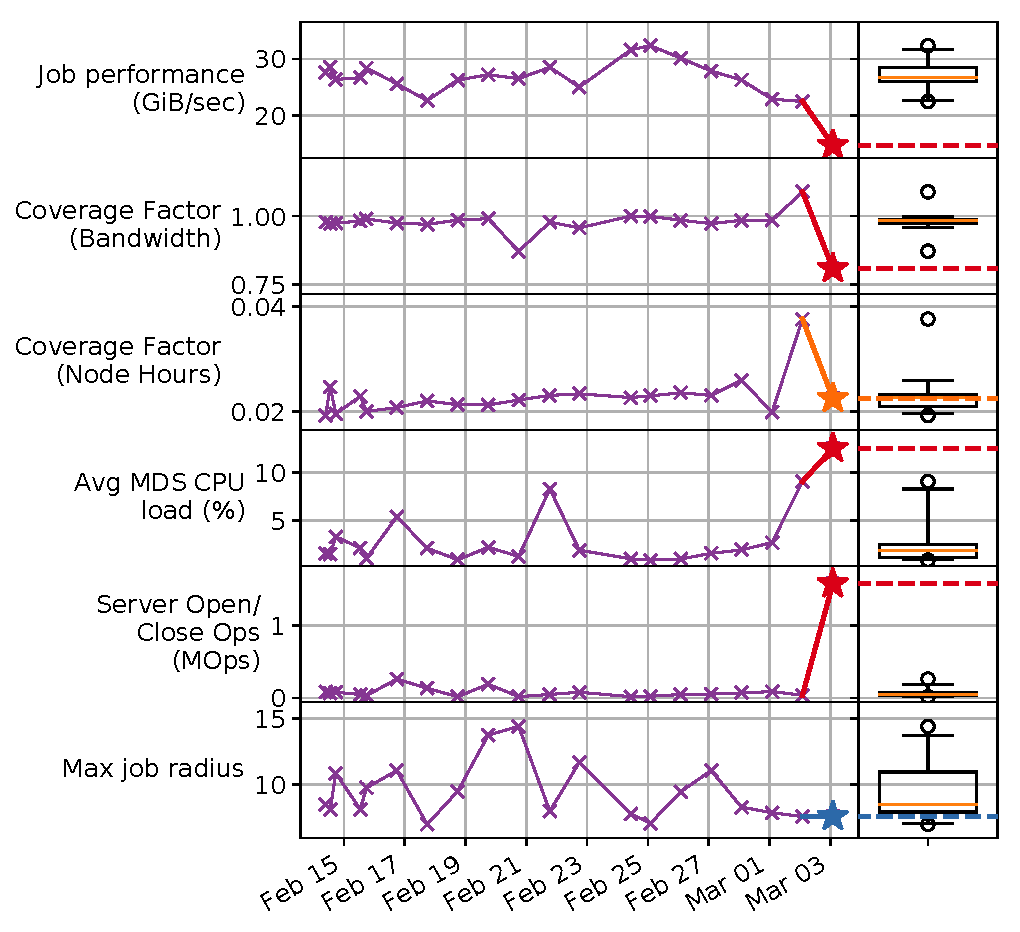
\includegraphics[width=1.0\columnwidth]{figs/umami-scratch2-hacc-write.pdf}
    \caption{UMAMI demonstrating the \emph{file system climate} of HACC write workloads on the Edison scratch2 file system compared to a most recent run, which showed highly unusual \emph{file system weather}.
    The left panes show the measurements from previous runs of the same motif, and the box plots in the right panes summarize the distribution of these metrics.
    The star denotes the metrics for the job of interest and is colored according to the quartile in which it falls (red being the worst quartile and blue the best).
    Box plot whiskers extend to the 5th and 95th percentiles, with outliers being denoted as circles.}
    \label{fig:umami-scratch2-hacc-write}
\vspace{-.2in}
\end{figure}

These $\mathit{CF}$ metrics, along with the system health and job topology data, let us contextualize performance anomalies and describe where a job's I/O performance falls on the spectrum of normalcy relative to jobs with similar motifs.
To concisely visualize all of this information and identify the metrics most likely contributing to abnormal performance, we display these data on a unified measurements and metrics interface (UMAMI) diagram.
UMAMI, demonstrated in Figure \ref{fig:umami-scratch2-hacc-write}, presents historic measurements (the I/O climate) and summarizes each metric's distribution in an accompanying box plot.
These time series plots terminate with the metrics for the job of interest and define the I/O weather at the time that job ran.
By overlaying this weather on the climate (dashed lines in the box plots), UMAMI provides a quick view of how each metric compared to the statistical distribution of past weather conditions and rapid differentiation of statistically rare events from long-term performance problems.% analogous to an extreme weather event.

In the remainder of this section, we identify different factors that do and do not contribute to I/O performance loss based on the holistic data analysis enabled by UMAMI.

% In the following sections, we illustrate how UMAMI can be applied to the problem of diagnosing poor performance of individual jobs in three case studies.

\subsection{Case Study: I/O Contention}

The UMAMI example in Figure \ref{fig:umami-scratch2-hacc-write} represents a HACC write test whose "Job performance" measurement and its value relative to previous instances of this type of job indicate statistically abnormal performance.
This poor performance was accompanied by an unusually low $\mathit{CF}_{\mathit{bw}}$ and high metadata load, highlighted as red dashed lines in the box plots that denote their place in the least-favorable quartile of past measurements.
The metrics corresponding to orange dashed lines ($\mathit{CF}_{\mathit{nodehrs}}$ and the number of overlapping jobs) fall in the second quartile, indicating that the number of concurrently running jobs and concurrently active compute nodes are too coarse-grained of metric to predict I/O performance.
The metric corresponding to blue dashed line, the maximum job radius, falls into the most favorable quartile for this problematic job and HACC has shown good I/O performance on much more topologically distributed node allocations.
Thus, we can attribute this HACC job's poor performance to I/O loads extrinsic to this job which competed for both bandwidth and metadata operation rates, and the number of concurrently running jobs and HACC's placement on Edison's dragonfly network had no discernible impact.

\subsection{Case Study: Metadata Load}

Figure \ref{fig:umami-mira-fs1-vpic-write} shows the UMAMI for a poorly performing VPIC workload.
$\mathit{CF}_{\mathit{bw}}$ is within normal parameters indicating regular levels of bandwidth contention.
Although $\mathit{CF}_{\mathit{IOPS}}$ is low, previous values have been equally low despite a lack of dramatic performance loss (e.g., on March 10).
The only metric that shows a unique, undesirable value is the number of \texttt{readdir(3)} operations handled by the file system.
This is indicative of an expansive file system traversal that was being performed at the same time as the job execution.
% The \emph{readdir(3)} metric was demonstrated to correlate moderately negatively with performance in Figure \ref{fig:correlation-table}.

\begin{figure}[t]
    \centering
    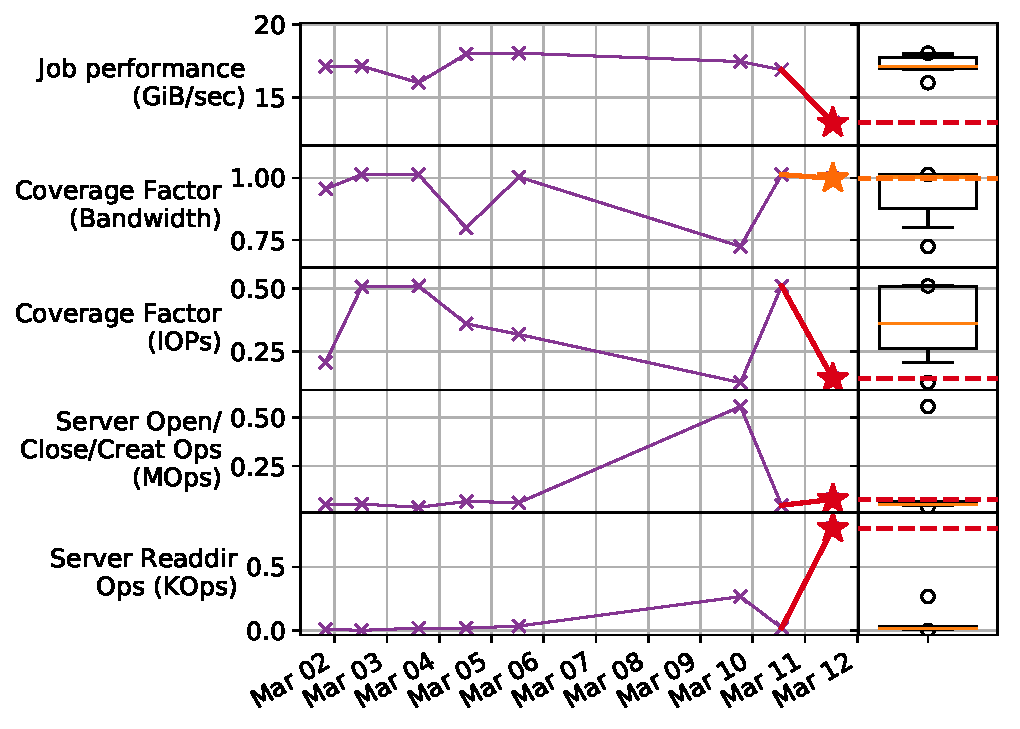
\includegraphics[width=1.0\columnwidth]{figs/umami-mira-fs1-vpic-write.pdf}
    \caption{UMAMI demonstrating the climate surrounding VPIC-IO write workloads on Mira compared to a most recent run, which showed highly unusual weather in the form of an excess of \texttt{readdir(3)} calls.
%   Significance of each pane and its contents are the same as explained in Figure \ref{fig:umami-scratch2-hacc-write}.
    }
    \label{fig:umami-mira-fs1-vpic-write}
\vspace{-.2in}
\end{figure}

%%%%%%%%%%%%%%%%%%%%%%%%%%%%%%%%%%%%%%%%%%%%%%%%%%%%%%%%%%%%%%%%%%%%%%%%%%%%%%%%
\subsection{Case Study: Storage Capacity}
%%%%%%%%%%%%%%%%%%%%%%%%%%%%%%%%%%%%%%%%%%%%%%%%%%%%%%%%%%%%%%%%%%%%%%%%%%%%%%%%

This holistic approach is also able to identify longer-term performance degradation.
Figure \ref{fig:umami-scratch3-hacc-write-long-term} shows the UMAMI view of such an event on Edison's scratch3 file system where coverage factors were not unusual despite an ongoing $2\times$ slowdown over the normal 50 GiB/sec.
The magnitude of performance loss followed the highest CPU load observed across all of the Lustre OSSes almost exactly, and this period coincided also with the scratch3 file system reaching critical levels of fullness.
Although such correlations cannot define causative relationships, these conditions indicated a relationship between critically full storage devices and CPU load (e.g., an increasing cost of scavenging empty blocks) that impacts application performance.
Incidentally, this behavior is consistent with known performance losses that result from Lustre OSTs filling~\cite{oral2014best}.
 
\begin{figure}[t]
    \centering
    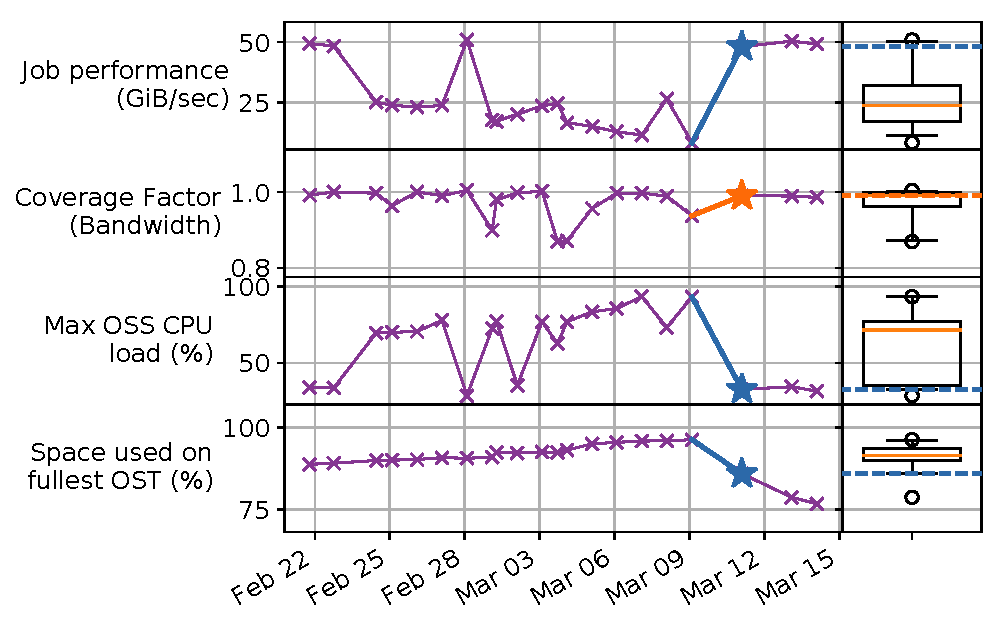
\includegraphics[width=1.0\columnwidth]{figs/umami-scratch3-hacc-write-long-term.pdf}
    \caption{UMAMI of HACC write performance on Edison's scratch3 file system showing a longer-term period of performance degradation that was associated with unusually high OSS CPU load.
%   Significance of each pane and its contents are the same as explained in Figure \ref{fig:umami-scratch2-hacc-write}.
    }
    \label{fig:umami-scratch3-hacc-write-long-term}
\vspace{-.2in}
\end{figure}
